\documentclass{scrbook}
\usepackage{graphicx} % Required for inserting images
\usepackage{tabularx} % Required for fixed width tables
\usepackage{scrlayer-scrpage} % Required for the subtitles
\usepackage{url} % Required for the URLs
\usepackage{hyperref} % Required for the URLs
\usepackage{listings} % Required for the code snippets

% Put the caption of the snippets at the bottom
\lstset{
    captionpos=b
}


\title{HyperText Markup Language}
\subtitle{Ambient intelligence course (A.Y. 2025/2026)\\Topic taught by Prof. Floriano Scioscia}
\author{Gabriele Colapinto}
\date{\today}

\begin{document}

\maketitle
\thispagestyle{empty}

{\Large\textbf{License}} \\
{Notes from Ambient intelligence (A.Y. 2025/2026) by Gabriele Colapinto. 
Course taught by professors Michele Ruta, Floriano Scioscia, Arnaldo Tomasino, Davide Loconte — 
Licensed under CC BY-NC 4.0.\\
\url{https://creativecommons.org/licenses/by-nc/4.0/}}

\vspace*{\fill}
\rule{\textwidth}{0.2pt}
\small{© 2025 Gabriele Colapinto \\
Released under the \href{https://creativecommons.org/licenses/by-nc/4.0/}{Creative Commons Attribution–NonCommercial 4.0 International License}}

\clearpage

\tableofcontents

\chapter{The Foundation of the Web: Defining HTML and its Core Principles}

HyperText Markup Language (HTML) is the foundational language for creating and structuring content on the World Wide Web. Before delving into its syntax and practical application, it is essential to understand its core principles and its collaborative relationship with other key web technologies. This section will define HTML, its purpose, and its place within the ecosystem that powers the modern web. \\

The World Wide Web Consortium (W3C) formally defines HTML as "the web's core language for creating content for everyone to use anywhere." This definition carries two profound implications. The phrase "for everyone" underscores a commitment to \textbf{accessibility}, ensuring that content is available to all users, including those with disabilities. The term "anywhere" highlights \textbf{interoperability}, emphasizing the need for content to be rendered consistently across a diverse range of devices, platforms, and user agents. \\

At its core, HTML is a language for creating \textbf{hypertext}, which is text that contains\\ hyperlinks—cross-references to other parts of the same document or to other resources on the web, such as pages or multimedia files. \\

To deliver a complete user experience, modern web content is understood from three distinct perspectives, each governed by a fundamental technology. Together, they form the trifecta that defines a modern web page: \\

\begin{itemize}
    \item
    \textbf{Structure:} HTML is the markup language used to define the logical structure of a web page as a hierarchy of elements. It labels pieces of content, such as headings, paragraphs, and tables, providing the essential scaffold upon which everything else is built.
    
    \item
    \textbf{Appearance:} Cascading Style Sheets (CSS) is the language that governs the appearance and presentation of the structured content. CSS controls aspects like colors, fonts, and layout, allowing for a clear separation between the document's structure and its visual styling.
    
    \item 
    \textbf{Behavior:} JavaScript is the programming language used to control the interactive behavior of the web page. It enables dynamic updates, user interactions, and complex application logic, transforming static documents into rich, responsive experiences.
\end{itemize}

Together, these three languages enable the creation of web content that is not only well-structured and accessible (HTML), but also visually engaging (CSS) and functionally interactive (JavaScript). \\

These technologies are requested, interpreted, and rendered by a \textbf{user agent}—the client software that acts on behalf of the user. While this term can apply to various clients, it most commonly refers to a web browser. This term originates from the HTTP specification, which defines the communication protocol between clients (user agents) and servers. With this foundational understanding, we can explore the historical evolution that shaped HTML into the powerful standard it is today.

\chapter{The Evolution of HTML Standards}

Understanding the history of HTML is crucial for appreciating its current design and best practices. Its journey from a simple language for sharing academic documents to a sophisticated platform for building complex web applications is a story of innovation, standardization, and adaptation. The evolution reflects a continuous effort to balance technical rigor with the practical needs of a rapidly expanding digital world. \\

The following milestones chronicle the development of HTML from its inception to its current state as a "Living Standard."

\begin{itemize}
    \item
    \textbf{1989:} At CERN, the European Organization for Nuclear Research, computer scientist Tim Berners-Lee proposes the project that would become the World Wide Web. He conceives of HTML as its primary publishing language, designed to facilitate the sharing of research documents among scientists.

    \item 
    \textbf{1997 (HTML 4.0):} This version marked a pivotal moment in web development with the introduction of Cascading Style Sheets (CSS). It was the first major step toward separating the structure of content (HTML) from its presentation (CSS), a principle that remains a cornerstone of modern web design.

    \item 
    \textbf{1999 (HTML 4.01):} This revision became a stable W3C recommendation, solidifying the standard for years to come. It formally deprecated many presentational elements and attributes, strongly encouraging developers to delegate all styling responsibilities to CSS.

    \item 
    \textbf{The XHTML Era (Early 2000s):} The W3C initiated an effort to reformulate HTML as a stricter, XML-based language known as XHTML. This push for strict, machine-readable syntax was directly fueled by the burgeoning vision of a "Semantic Web," where automated agents could process content—a vision articulated by Tim Berners-Lee in his seminal 1999 article in Scientific American. However, this initiative ultimately failed to gain widespread adoption. The primary reason was the sheer volume of existing, syntactically incorrect HTML on the web. Web browsers were designed to be permissive, rendering malformed code as best they could. Consequently, web authors and tool developers had no compelling reason to undertake the massive effort of fixing their existing content to conform to XHTML's rigid rules.

    \item 
    \textbf{2014 (HTML5):} After the stagnation of the XHTML era, HTML5 emerged as the next major evolution. Published as a W3C recommendation, it introduced a host of new elements and application programming interfaces (APIs) designed to support modern web applications, including native multimedia (\texttt{<video>}, \texttt{<audio>}) and advanced form controls.

    \item 
    \textbf{2019 (HTML Living Standard):} The standardization model shifted away from version numbers. The responsibility for maintaining the HTML standard was transferred to the Web Hypertext Application Technology Working Group (WHATWG). As a "Living Standard," HTML now evolves continuously. This model gives greater weight to technology providers, including major browser vendors and developers of widely-used authoring tools and libraries, ensuring that the standard reflects practical implementation and industry acceptance.
\end{itemize}

The failed XHTML experiment taught the web community a critical lesson: new standards cannot succeed without the acceptance and participation of the key stakeholders. The evolution of web technologies is driven by a "triangle" of influence between \textbf{tool providers} (e.g., browser vendors, authoring tools), \textbf{web developers} (who create the content), and \textbf{users} (whose needs and behaviors shape demand). The successful adoption of any new standard requires that all three of these groups move forward in concert. This historical context leads us to the fundamental structure that underlies every HTML document.

\begin{figure}
    \centering
    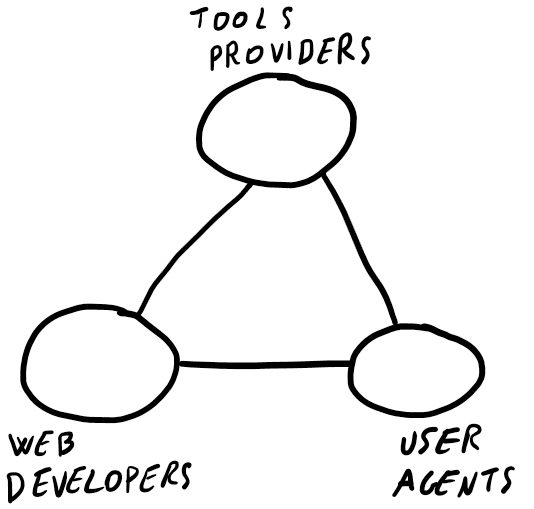
\includegraphics[width=0.5\linewidth]{Images/Triangle.png}
    \caption{Web technologies stakeholders triangle}
\end{figure}

\chapter{Anatomy of an HTML Document}

\begin{figure}
    \centering
    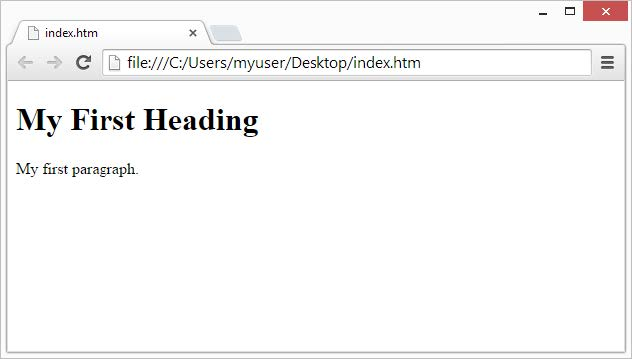
\includegraphics[width=0.5\linewidth]{Images/Page_example.jpg}
    \caption{Web page example (The tab title should be "Page Title" instead of "index.html")}
\end{figure}

All HTML documents, from the simplest page to the most complex web application, adhere to a fundamental structure. This structure consists of a few essential components that define the document and organize its content. This section will dissect that basic anatomy. \\

The following code block illustrates the essential structure of an HTML page, with comments explaining each part:

\begin{lstlisting}[language=HTML, caption={Essential structure of an HTML page}]
<!DOCTYPE html>
<!-- The DOCTYPE declaration defines the document type and version. -->
<html>
  <!-- The <html> element is the root of the entire document. -->
  <head>
    <!-- The <head> element contains meta-information about the page. -->
    <title>Page Title</title>
    <!-- The <title> element specifies the title shown in the browser tab. -->
  </head>
  <body>
    <!-- The <body> element contains the visible content of the page. -->
    <h1>My First Heading</h1>
    <p>My first paragraph.</p>
  </body>
</html>
\end{lstlisting}

The core components shown in this example form the skeleton of every web page:

\begin{itemize}
    \item 
    \texttt{\textbf{<!DOCTYPE html>:}} This is the document type declaration. It must be the very first thing in the document. Its purpose is to instruct the browser on the version of HTML being used, which ensures the page is rendered correctly according to modern web standards.

    \item 
    \texttt{\textbf{<html>:}} This is the root element of the page. It acts as a container that encapsulates all other HTML elements.

    \item 
    \texttt{\textbf{<head>:}} This element contains metadata—data about the HTML document itself. This information is not displayed directly on the rendered page but is processed by the browser and other services (like search engines). It typically includes the page title, character set definitions, and links to external resources like CSS stylesheets and JavaScript files.

    \item 
    \texttt{\textbf{<body>:}} This element contains all the visible content of the web page. Everything that the user sees in the browser window—such as headings, paragraphs, images, links, and tables—is placed within the \textless body\textgreater tags.

    \item 
    \texttt{\textbf{<h1>:}} This tag defines a large heading. There are 6 heading tags in total ranging from \textless h1\textgreater (the largest) to \textless h6\textgreater (the smallest).

    \item 
    \texttt{\textbf{<p>:}} This tag defines a paragraph.
\end{itemize}

Having established this basic structure, we will now examine the DOCTYPE declaration in greater detail to understand its critical function.

\chapter{The Document Type Declaration (DOCTYPE)}

The Document Type Declaration (DOCTYPE) plays a critical role in how a web page is rendered. Its primary function is to inform the user agent of the specific version of HTML the document conforms to. Including a correct DOCTYPE prevents the browser from switching to "quirks mode," a backward-compatibility mode that mimics the non-standard rendering behaviors of older browsers. By declaring a modern DOCTYPE, you ensure the browser renders the page according to established web standards, leading to more predictable and consistent results.

\section{HTML 4.01 DTDs}

\begin{figure}
    \centering
    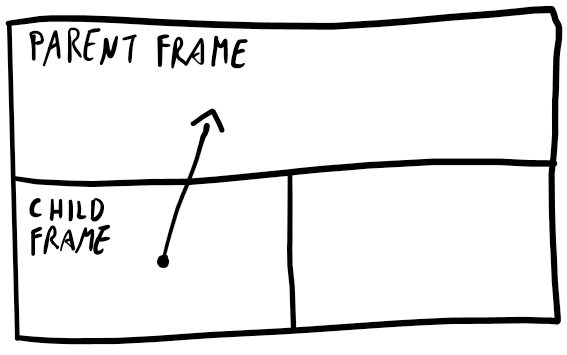
\includegraphics[width=0.5\linewidth]{Images/Frames.png}
    \caption{Example of web page with frames}
\end{figure}

Because HTML 4.01 was formally based on Standard Generalized Markup Language (SGML), its DOCTYPE required a reference to a Document Type Definition (DTD). The DTD specifies the rules for the markup language, so the browser can parse the content correctly. Three DTDs were available for HTML 4.01:

\begin{itemize}
    \item 
    \textbf{Strict:} \texttt{<!DOCTYPE HTML PUBLIC "-//W3C//DTD HTML 4.01//EN" \\ "http://www.w3.org/TR/html4/strict.dtd">} \\
    
    This was the most rigorous DTD. It excluded all deprecated elements and presentational attributes (such as \texttt{<font>}). Its use enforced a clean separation of structure (HTML) from presentation, with all styling intended to be handled by CSS.

    \item 
    \textbf{Transitional:} \texttt{<!DOCTYPE HTML PUBLIC "-//W3C//DTD HTML 4.01 Transitional//EN" \\ "http://www.w3.org/TR/html4/loose.dtd">} \\

    This DTD includes everything in the Strict DTD but also permits the use of some deprecated elements and attributes. It was designed to provide a transitional path for developers, allowing for backward compatibility with older web content that mixed structure and presentation.

    \item 
    \textbf{Frameset:} \texttt{<!DOCTYPE HTML PUBLIC "-//W3C//DTD HTML 4.01 Frameset//EN" \\ "http://www.w3.org/TR/html4/frameset.dtd">} \\

    This DTD is an extension of the Transitional DTD that also supports the use of frames to divide the browser viewport into multiple, independent sub-windows. Frames are now obsolete because they created a poor user experience, such as breaking the browser's "back" button functionality and making it impossible to bookmark or share a link to a specific state of the page.
\end{itemize}

\section{The Modern HTML5 DOCTYPE}

HTML5 is not based on SGML, which has greatly simplified the declaration. It no longer requires a reference to a DTD. The modern, simplified syntax is all that is needed to ensure standards-mode rendering in all current browsers: \\

\texttt{<!DOCTYPE html>} \\

This streamlined declaration is one of the many practical improvements introduced with HTML5. With the document type defined, we can now turn to the fundamental building blocks contained within the structure.

\chapter{Core Concepts: Tags, Elements, Entities, and Attributes}

The structure of an HTML document is built from a few fundamental concepts. \textbf{Elements} are the building blocks of the page, which are in turn defined by \textbf{tags}. \textbf{Attributes} provide additional information about those elements, modifying their behavior or providing metadata. Understanding these core components is essential to writing HTML.

\section{ Elements and Tags}

An HTML \textbf{element} is an individual component of a web page. It typically consists of a start tag, some content, and an end tag. For example, \texttt{<p>This is a paragraph.</p>} is a paragraph element. \\

\textbf{Tags} are the keywords enclosed in angle brackets (\texttt{<>}) that define the element. The start tag marks the beginning of an element (e.g., \texttt{<p>}), and the end tag, which includes a forward slash, marks its end (e.g., \texttt{</p>}). A key feature inherited from SGML is that HTML tags are \textbf{case-insensitive}, meaning \texttt{<p>} is treated the same as \texttt{<P>}. There are also self-closing tags like \texttt{<br/>} that do not require a closing tag.

\section{HTML Entities}

HTML entities are special codes used to represent reserved characters (which might otherwise be interpreted as HTML code) or special symbols. They can be referenced by name or number. The five most frequently used entities are:

\begin{table}[h!]
    \centering
    \begin{tabularx}{\textwidth}{|X|X|X|} \hline
        \textbf{Character} & \textbf{Entity Name} & \textbf{Entity Number} \\ \hline

        \textless & \&lt; & \&\#60; \\
        \hline

        \textgreater & \&gt; & \&\#62; \\
        \hline

        \& & \&amp; & \&\#38; \\
        \hline

        " & \&quot; & \&\#34; \\
        \hline

        ' & \&apos; & \&\#39; \\
        \hline
    \end{tabularx}
    \caption{Selection of HTML entities with name and number}
\end{table}

\section{Attributes}

Attributes are name-value pairs specified within the start tag of an element that provide additional information or modify the element's default behavior. While many attributes are specific to certain elements, several \textbf{Global Attributes} can be used with any HTML element.

\begin{table}[h!]
    \centering
    \begin{tabularx}{\textwidth}{|p{5em}|X|} \hline
        \textbf{Attribute} & \textbf{Description}  \\ \hline

        \texttt{id} &
        Specifies a unique identifier for an element within the document.
        \\ \hline

        \texttt{class} &
        Assigns one or more class names to an element, used for styling with CSS or selecting with JavaScript. Multiple elements can share the same class.
        \\ \hline

        \texttt{style} &
        Applies inline CSS rules directly to a single element. Its use is strongly discouraged in modern practice as it violates the core principle of separating structure from presentation, leading to less maintainable code.
        \\ \hline

        \texttt{lang} &
        Specifies the language of the element's content.
        \\ \hline

        \texttt{title} &
        Provides extra information about an element, which is typically displayed as a tooltip when the user's mouse hovers over the element.
        \\ \hline
    \end{tabularx}
    \caption{Selection of HTML entities with name and number}
\end{table}

\section{Event Attributes}

Event attributes serve as a bridge to interactivity, allowing you to trigger JavaScript functions in response to user actions. For example, the \texttt{onkeydown} attribute can be added to an input field to execute a specific function whenever a user presses a key within that element. Many categories of events exist, including Mouse events (\texttt{onclick}, \texttt{onmouseover}), Form events (\texttt{onsubmit}), and Window events (\texttt{onload}), enabling rich, dynamic user experiences. From these individual building blocks, we can now examine how elements are organized into the two major layout categories.

\chapter{Document Layout: Block and Inline Elements}

In the model used by web browsers, every visible HTML element is rendered as a rectangular box on the page. This concept, known as the CSS box model, is fundamental to understanding web page layout. HTML elements are categorized into two main layout types based on their default display behavior: block and inline.

\begin{itemize}
    \item
    \textbf{Block-level Elements:} These elements form the major structural components of a page. By default, they always start on a new line and expand to take up the full width of their container. They can contain other block-level elements as well as inline elements. This allows for a nested, hierarchical structure, much like a matryoshka doll, where larger containers hold progressively smaller ones. Primary examples include the \texttt{<div>} (a generic container), \texttt{<p>} (paragraph), and the heading elements \texttt{<h1>} through \texttt{<h6>}.

    \item 
    \textbf{Inline Elements:} These elements are designed to be part of the flow of text within a block-level element. They do not start on a new line and only take up as much width as their content requires. They can contain text and other inline elements but cannot contain block-level elements. Primary examples include \texttt{<span>} (a generic inline container), \texttt{<a>} (anchor/hyperlink), and \texttt{<img>} (image).
\end{itemize}

Understanding this distinction is key to controlling document flow and layout. However, modern web development emphasizes not just how an element \textit{looks}, but what it \textit{means}—a concept known as semantic HTML.

\begin{figure}
    \centering
    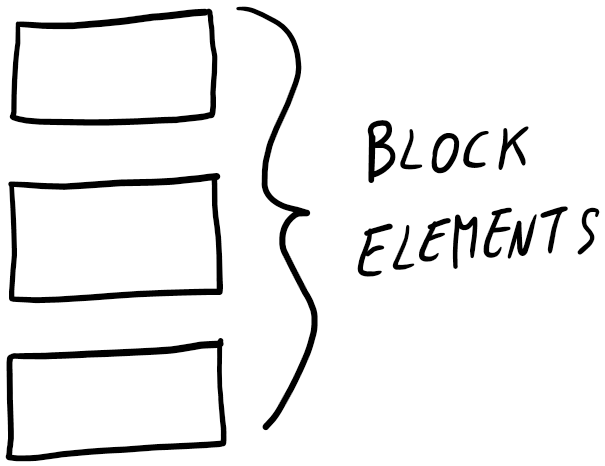
\includegraphics[width=0.5\linewidth]{Images/Block_elements.png}
    \caption{HTML block elements}
\end{figure}

\begin{figure}
    \centering
    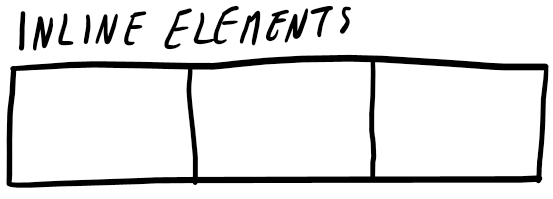
\includegraphics[width=0.5\linewidth]{Images/Inline_elements.png}
    \caption{HTML inline elements}
\end{figure}

\begin{figure}
    \centering
    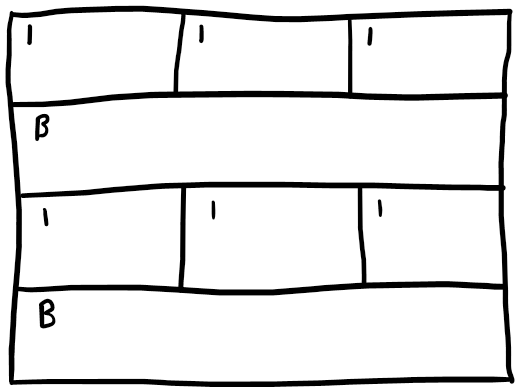
\includegraphics[width=0.5\linewidth]{Images/Elements_example.png}
    \caption{Example of HTML page containing both block and inline elements}
\end{figure}

\chapter{Semantic HTML: Writing for Meaning}

A philosophical evolution in web development has been the shift toward semantic \textbf{HTML}, where elements are chosen based on the meaning of the content they enclose. This stands in contrast to the older, purely presentational approach, often characteristic of the "What you see is what you get" (WYSIWYG) paradigm, where tags like \texttt{<b>} (bold) were used simply to style text. The modern methodology recognizes that separating the \textit{meaning} of content from its \textit{presentation} creates a more robust, accessible, and future-proof web. Using semantic elements provides several strategic benefits:

\begin{itemize}
    \item
    \textbf{Improved Accessibility:} Assistive technologies, such as screen readers for visually impaired users, rely on semantic markup to interpret the structure and importance of content. An \texttt{<h1>} tag clearly signals the main heading of the page, whereas a generic \texttt{<div>} styled to look large provides no such context.

    \item
    \textbf{Better Search Engine Optimization (SEO):} Search engines analyze the semantic structure of a page to understand its content hierarchy and relevance. Using tags like \texttt{<strong>} to indicate importance helps search engines identify key terms, potentially improving the page's ranking in search results.

    \item
    \textbf{Clearer, More Maintainable Code:} Semantic markup makes the HTML source code more readable and self-documenting. A developer can immediately understand the purpose of a \texttt{<nav>} or \texttt{<footer>} element, making the codebase easier to maintain and update.
\end{itemize}

\begin{figure}
    \centering
    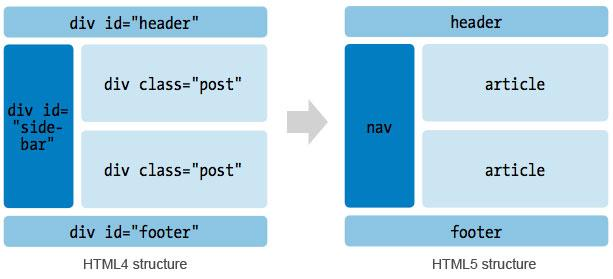
\includegraphics[width=0.6\linewidth]{Images/Structure_with_semantic_tags.jpg}
    \caption{HTML page structure without and with semantic tags}
\end{figure}

The following table contrasts some older, presentational tags with their modern semantic HTML5 equivalents, highlighting the shift from visual instruction to meaningful description.

\begin{table}[h!]
    \centering
    \begin{tabularx}{\textwidth}{|X|X|X|}
        \hline
        \textbf{Original Tag (Presentational)} & \textbf{Modern Tag (Semantic)} & \textbf{Semantic Meaning \& Interpretation} \\
        \hline

        \texttt{<b>} & \texttt{<strong>} &
        Indicates that the enclosed text has strong importance or urgency. Interpreted by search engines as a signal of semantic emphasis. \\
        \hline

        \texttt{<i>} & \texttt{<em>} &
        Indicates emphasized text, representing a different tone or voice. Signals contextual emphasis to assistive technologies. \\
        \hline

        \texttt{<s>} or \texttt{<strike>} & \texttt{<del>} &
        Represents text that has been deleted or is no longer valid. Useful for tracking changes in documents. \\
        \hline

        \texttt{<u>} & \texttt{<ins>} &
        Represents text that has been inserted into the document. Semantically marks an addition. \\
        \hline
    \end{tabularx}
    \caption{Comparison of original tags and modern tags}
\end{table}

By using elements like  \texttt{<h1>} through  \texttt{<h6>} for headings and  \texttt{<strong>} for important text, developers create a clear content hierarchy that can be understood by both machines and humans. This meaningful structure is built from a core set of common content elements.

\chapter{Essential Content Elements}

While the HTML specification includes a vast number of elements, a relatively small subset forms the foundation of most content published on the web. A practical understanding of these essential elements is the first step toward creating well-structured web pages.

\section{Headings}

These six elements are used to define a hierarchical structure of titles and subtitles for a document. The \texttt{<h1>} element represents the most important heading (typically the main page title), while \texttt{<h6>} represents the least important. Using headings correctly is crucial for creating a logical document outline that is beneficial for both accessibility and SEO.

\section{Paragraphs}

The \texttt{<p>} element is the fundamental element for grouping sentences and defining a paragraph of text. Browsers automatically add vertical space before and after each paragraph, visually separating blocks of text.

\section{Anchors}

The anchor (\texttt{<a>}) element is used to create hyperlinks, the defining feature of hypertext. The destination of the link is specified by its \texttt{href} (hypertext reference) attribute, which can point to another web page, a location within the same page, or any other web resource.

\section{Lists}

HTML provides two main types of lists for grouping and organizing related items, each serving a different structural purpose.

\begin{itemize}
    \item
    \textbf{Unordered Lists:} The \texttt{<ul>} element is used to create a list of items where the order is not important. Each item in the list is defined with an \texttt{<li>} (list item) element. By default, browsers render these as a bulleted list.

    \item
    \textbf{Ordered Lists:} The \texttt{<ol>} element creates a list where the order of items is meaningful. As with unordered lists, each item is defined with an \texttt{<li>} element. The browser renders this as a numbered list by default. The numbering style can be changed using the type attribute.
\end{itemize}

\begin{table}[h!]
    \centering
    \begin{tabularx}{\textwidth}{|p{5em}|X|} \hline
        \texttt{type} Value & Description \\ \hline
    
        \texttt{1} & Numbers (default) \\ \hline
    
        \texttt{A} & Uppercase letters \\ \hline
    
        \texttt{a} & Lowercase letters \\ \hline
    
        \texttt{I} & Uppercase Roman numerals \\ \hline
    
        \texttt{i} & Lowercase Roman numerals \\ \hline
    \end{tabularx}
    \caption{Ordered lists numbering types}
\end{table}

\section{Hyperlinks}

Hyperlinks are a foundational feature of hypertext and are created using the anchor (\texttt{<a>}) tag. This element turns text or other content into a clickable link that navigates the user to another document or a specific part of the current document. Its behavior is primarily controlled by two essential attributes.

\begin{itemize}
    \item
    \textbf{href:} Specifies the destination Uniform Resource Name (URN) of the link. The acronym stands for 'hypertext reference'.

    \item
    \textbf{target:} Determines where the linked document will open. Key values include:
    
    \begin{itemize}
        \item
        \textbf{\_blank:} Opens the link in a new window or tab.

        \item
        \textbf{\_self:} Opens the link in the same window/tab (this is the default behavior).

        \item
        \textbf{\_parent:} Opens the link in the parent frame.

        \item
        \textbf{\_top:} Opens the link in the full body of the window.
    \end{itemize}
    
     \textit{Note: \_parent and \_top are rarely used in modern development due to the deprecation of frames in HTML5.}

     It is also possible to create \textbf{bookmarks}, or internal page links, that allow users to jump to a specific section of the same page. This is achieved by assigning a unique \texttt{id} attribute to the target element and referencing it in the \texttt{href} attribute with a hash (\texttt{\#}) prefix (e.g., \texttt{<a href="\#news">}).
\end{itemize}

\section{Images}

The image (\texttt{<img>}) tag is used to embed images directly into a web page. It is an empty element, meaning it contains attributes only and does not have a closing tag.

\begin{table}[h!]
    \centering
    \begin{tabularx}{\textwidth}{|p{5em}|X|} \hline
        \textbf{Attribute} & \textbf{Description} \\ \hline
    
        \texttt{src} & Specifies the URL or path to the image file. This attribute is mandatory. \\ \hline
    
        \texttt{alt} & Provides \textbf{alternate text} for the image. This text is crucial for accessibility, as it is displayed by devices that cannot render images and read by screen readers for users who cannot see them. \\ \hline
    
        \texttt{width} & Sets the width of the image in pixels. \\ \hline
    
        \texttt{height} & Sets the height of the image in pixels. \\ \hline
    \end{tabularx}
    \caption{Image attributes}
\end{table}

While \texttt{width} and \texttt{height} attributes can be used to define an image's dimensions, the preferred modern approach is to control sizing with CSS for greater flexibility and maintainability. If dimensions are not specified, the image will be displayed at its native size.

\section{Object}

The \texttt{<object>} HTML element represents an external resource, which can be treated as an image, a nested browsing context, or a resource to be handled by a plugin.

\section{Tables}

The \texttt{<table>} element is used to organize and display data in a two-dimensional, tabular format. The structure of a table is built with a set of core, nested elements:

\begin{itemize}
    \item
    \textbf{\texttt{<tr>} (Table Row):} Defines a row within the table.

    \item
    \textbf{\texttt{<th>} (Table Header):} Defines a header cell, which is typically displayed as bold and centered. It is used to label columns or rows.

    \item
    \textbf{\texttt{<td>} (Table Data):} Defines a standard data cell within a table row.
\end{itemize}

For example, the following code produces the table shown in figure 8.1.

\begin{lstlisting}[language=HTML, caption={HTML table example code}]
    <table border="2">
        <tr>
            <th>Firstname</th>
            <th>Lastname</th>
            <th>Age</th>
        </tr>
        <tr>
            <td>Jill</td>
            <td>Smith</td>
            <td>50</td>
        </tr>
        <tr>
            <td>Eve</td>
            <td>Jackson</td>
            <td>94</td>
        </tr>
        <tr>
            <td>John</td>
            <td>Doe</td>
            <td>80</td>
        </tr>
    </table>
\end{lstlisting}

\begin{figure}
    \centering
    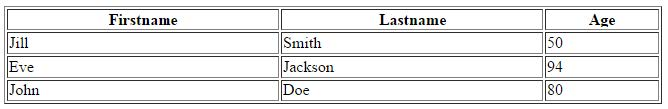
\includegraphics[width=0.7\linewidth]{Images/Table_example.jpg}
    \caption{HTML table example}
\end{figure}

For more complex data layouts, a single cell can be made to span multiple columns or rows using the \texttt{colspan} and \texttt{rowspan} attributes, respectively. For instance, \texttt{<td colspan="2">} would create a data cell that occupies the width of two columns.

\section{Forms}

The \texttt{<form>} element serves as a container for various input controls, allowing a website to collect data from users. Key attributes of the \texttt{<form>} tag define how the data is handled upon submission:

\begin{itemize}
    \item
    \textbf{\texttt{action}:} Specifies the destination URL where the form data will be sent for processing when the form is submitted. This is a mandatory attribute.

    \item
    \textbf{\texttt{method}:} Defines the HTTP method to be used for transmitting the data. The two possibilities are \texttt{GET} and \texttt{POST}. With the \texttt{GET} method (the default), form data is appended to the URL as a list of key-value pairs (e.g., \texttt{?name1=value1\&name2=value2)}. Special characters in the data are automatically URL-encoded by the browser to ensure the URL remains valid.

    \item
    \textbf{\texttt{enctype}:} Specifies how the form data should be encoded when it is submitted. The default is \texttt{application/x-www-form-urlencoded}, which is suitable for the \texttt{GET} method.
\end{itemize}

The most versatile element within a form is \texttt{<input>}, whose function changes based on its \texttt{type} attribute. Every input control must have a \texttt{name} attribute, which acts as the key in the submitted key-value pair. The function of the \texttt{value} attribute depends on the input \texttt{type}: for text fields it can define a default value, while for buttons it often defines the visible text.

\begin{table}[h!]
    \centering
    \begin{tabularx}{\textwidth}{|p{7em}|X|} \hline
        \texttt{type} Attribute & Function \\ \hline
    
        \texttt{text} & Creates a single-line text input field. \\ \hline
    
        \texttt{radio} & Creates a radio button, used in a group where only one option can be selected. \\ \hline

        \texttt{checkbox} & Creates a box that is checked (ticked) when activated. \\ \hline
    
        \texttt{submit} & Creates a button that submits the form. The text displayed on the button is defined by its \texttt{value} attribute (e.g., \texttt{<input type="submit" value="Send">}). \\ \hline
    \end{tabularx}
    \caption{Input types}
\end{table}

Other important form elements include:

\begin{itemize}
    \item
    \textbf{\texttt{<textarea>}:} Provides a multi-line text input control.

    \item
    \textbf{\texttt{<label>}:} Defines a label for a form control, which improves accessibility by associating descriptive text with an input field.

    \item
    \textbf{\texttt{<select>}:} Creates a drop-down list from which users can choose one or more options.

    \item
    \textbf{\texttt{<button>}:} Defines a clickable button that can be used for actions other than form submission, often in conjunction with JavaScript.
\end{itemize}

The following form example HTML code produces the form shown in figure 8.2.

\begin{lstlisting}[language=HTML, caption={HTML form example}]
    <form action="action_page.php">
        First name: <input type="text" name ="firstname" value="Mickey">
        Last name: <input type="text" name="lastname" value="Mouse">
        <input type="submit" value="Submit">
    </form>
\end{lstlisting}

\begin{figure}
    \centering
    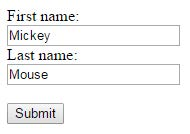
\includegraphics[width=0.5\linewidth]{Images/Form_example.jpg}
    \caption{HTML form example}
\end{figure}

\section{Integrated Multimedia: Audio and Video}

HTML5 introduced the \texttt{<audio>} and \texttt{<video>} elements as a standard way to embed media directly into a webpage, replacing the older, plugin-based methods like Adobe Flash. This provided a more interoperable, accessible, and easier-to-program solution for multimedia content. \\

The \texttt{<video>} tag is particularly powerful, allowing developers to provide multiple media formats to ensure broad browser compatibility. This is done by nesting \texttt{<source>} elements, each pointing to a different file format—such as MP4 or OGG, which is a container format rather than a specific encoding—within the \texttt{<video>} tag. The browser will then use the first format it supports and, if it doesn't support any of the given formats, it shows the error message written after the \texttt{<source>} tags.

\begin{lstlisting}[language=html]
<video controls>
    <source src="movie.mp4" type="video/mp4">
    <source src="movie.ogg" type="video/ogg">
    Your browser does not support the video tag.
</video>
\end{lstlisting}

Key attributes include \texttt{controls}, which adds standard video controls like play, pause, and volume, and \texttt{alt}, which provides alternative text for accessibility. The \texttt{autoplay} attribute exists to start a video automatically, but its use is considered a disruptive practice, especially on mobile devices where it can lead to unwanted data consumption.

\section{Advanced Graphics: SVG and Canvas}

HTML5 also introduced two new elements for rendering advanced graphics directly in the browser: \texttt{<svg>} and \texttt{<canvas>}.

\begin{itemize}
    \item \textbf{SVG (Scalable Vector Graphics):} SVG is an XML-based format for defining vector-based graphics. Unlike raster image formats (like JPG or PNG) that are composed of pixels, vector graphics are defined by mathematical primitives like lines and curves. The primary advantage of SVG is that images are infinitely \textbf{scalable}; they can be resized to any dimension without losing quality or becoming pixelated.
    \item \textbf{Canvas:} The \texttt{<canvas>} element provides a container, or "drawing area," where graphics can be rendered on the fly using JavaScript. Unlike the static nature of an \texttt{<img>} or \texttt{<svg>} tag, a canvas is a dynamic surface whose content can be programmatically changed in response to user interaction or other events. This makes it ideal for interactive applications, data visualizations, and games.
\end{itemize}

\begin{figure}
    \centering
    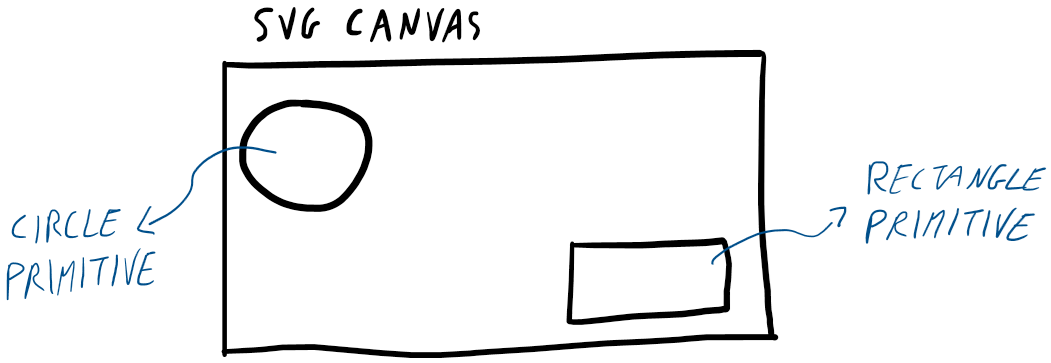
\includegraphics[width=0.5\linewidth]{Images/Canvas_example.png}
    \caption{Canvas example}
\end{figure}

\chapter{HTML5 guidelines to write a well-formed document}

HTML5 specifies a set of guidelines and best practices to write robust and interoperable documents. Following these rules is not mandatory but is highly recommended to achieve the desired end result. Not following these rules can cause the page to not be shown as intended because the browser uses a \textbf{best effort policy}. This means that, in case of malformed document, it tries to guess the intention of the web developer to render the page. This is a design decision meant to allow flexibility at the cost of computational effort from the browser. Writing a well-formed document allows the browser to render the page without making any guesswork resulting in a faster and less power-consuming rendering.

\begin{enumerate}
    \item 
    \parbox[t]{\linewidth}{
        \textbf{Always declare the document type as the first line in your document.} \\
        This is to make sure that the browser knows what type of document it is rendering.
    }

    \item 
    \parbox[t]{\linewidth}{
        \textbf{Use lower-case element and attribute names.} \\
        This guideline is confusing because the careful reader read that HTML tags are case insensitive in previous chapters. The truth is that this guideline does not enforce a functional requirement in the context of HTML itself. Instead, it is derived from the fact that HTML documents can also be serialized as XML (XHTML), where element and attribute names are \textit{case sensitive}. So, basically, this guideline enforces clarity in the parsing process and backwards compatibility.
    }

    \item 
    \parbox[t]{\linewidth}{
        \textbf{Explicitly close non-void HTML elements.} \\
        While HTML5 allows void elements such as \texttt{<img>} or \texttt{<br>} to be unclosed, explicitly closing all non-void elements improves clarity and compatibility with XML-based parsers.
    }

    \item 
    \parbox[t]{\linewidth}{
        \textbf{Quote attribute values.} \\
        This syntactic convention allows to have attributes values which contain a blank space. For instance, the alternative text of an image: \\
        \texttt{<img src="html5.gif" alt="HTML5 Icon" width="128" height="128">}.
    }

    \item 
    \parbox[t]{\linewidth}{
        \textbf{Add the "alt" attribute to images.} \\
        This guideline exists for accessibility purposes. Screen readers cannot display an image, they can only read its alternative text.
    }

    \item 
    \parbox[t]{\linewidth}{
        \textbf{Avoid spaces around equal signs and angular brackets.} \\
        This guideline improves readability and consistency of the markup, but it does not affect HTML parsing correctness.
    }

    \item 
    \parbox[t]{\linewidth}{
        \textbf{Use blank lines and indentation.} \\
        This guideline favors human readability of the document. A legible document makes the tag hierarchy and the functional blocks of the document evident to the eyes of the human reader. 
    }

    \item 
    \parbox[t]{\linewidth}{
        \textbf{Do not omit \texttt{<html>} and \texttt{<body>} tags.} \\
        Although browsers automatically insert missing \texttt{<html>} and \texttt{<body>} elements, explicitly declaring them improves document clarity and interoperability. 
    }

    \item 
    \parbox[t]{\linewidth}{
        \textbf{Use the \texttt{<title>} tag in the head of the document.} \\
        One might think that using the \texttt{<title>} tag is not necessary because the browser can use the name of the file as the title displayed in the tab. The problem is that this reasoning does not take into account the fact that the name of the page is not merely a label and a web browser is not the only user agent that can read the page. The \texttt{<title>} tag is the main semantic attribute of the page and is used to identify it. This makes the work of SEO tools easier, allows screen readers to read the name of the page before its content and makes the search history of the browser clearer. Without the \texttt{<title>} tag it is more difficult to find the page on the Internet, it is not possible for a visually impaired user to know the title of the web page and the web page is harder to detect in the search history.
    }

    \item 
    \parbox[t]{\linewidth}{
        \textbf{Use and link style sheets (CSS) with a simple syntax.} \\
        It is preferable to create external style sheets and link them to the document using a simple syntax such as: \texttt{<link rel="stylesheet" href="styles.css">}. This separates the structure of the web page from its style favoring maintainability and scalability of the project. This favors maintainability by allowing to change the style sheet without touching the HTML file and favors scalability because this approach allows to import other documents.
    }

    \item 
    \parbox[t]{\linewidth}{
        \textbf{Load JavaScript at the end of HTML (when possible).} \\
        The JavaScript execution environment is single-threaded, and synchronous scripts can block HTML parsing and rendering. Inserting or loading a script before the \texttt{<body>} tag would make the rendering process execute the script before rendering and showing the page. This creates a latency proportional to the execution time of the scripts. A slow loading page is unpleasant to the eyes of the end user so, when devising the structure of the web page, it's crucial for us developers to make sure that the body of the document is loaded as quickly as possible.
    }
\end{enumerate}

\end{document}
